\RequirePackage[l2tabu, orthodox]{nag}
\documentclass[version=3.21, pagesize, twoside=off, bibliography=totoc, DIV=calc, fontsize=12pt, a4paper]{scrartcl}
%Permits to copy eg x ⪰ y ⇔ v(x) ≥ v(y) from PDF to unicode data, and to search. From pdfTeX users manual. See https://tex.stackexchange.com/posts/comments/1203887.
	\input glyphtounicode
	\pdfgentounicode=1
%Latin Modern has more glyphs than Computer Modern, such as diacritical characters. fntguide commands to load the font before fontenc, to prevent default loading of cmr.
	\usepackage{lmodern}
%Encode resulting accented characters correctly in resulting PDF, permits copy from PDF.
	\usepackage[T1]{fontenc}
%UTF8 seems to be the default in recent TeX installations, but not all, see https://tex.stackexchange.com/a/370280.
	\usepackage[utf8]{inputenc}
%Provides \newunicodechar for easy definition of supplementary UTF8 characters such as → or ≤ for use in source code.
	\usepackage{newunicodechar}
%Text Companion fonts, much used together with CM-like fonts. Provides \texteuro and commands for text mode characters such as \textminus, \textrightarrow, \textlbrackdbl.
	\usepackage{textcomp}
%St Mary’s Road symbol font, used for ⟦ = \llbracket.
	\usepackage{stmaryrd}
%Solves bug in lmodern, https://tex.stackexchange.com/a/261188; probably useful only for unusually big font sizes; and probably better to use exscale instead. Note that the authors of exscale write against this trick.
	%\DeclareFontShape{OMX}{cmex}{m}{n}{
		%<-7.5> cmex7
		%<7.5-8.5> cmex8
		%<8.5-9.5> cmex9
		%<9.5-> cmex10
	%}{}
	%\SetSymbolFont{largesymbols}{normal}{OMX}{cmex}{m}{n}
%More symbols (such as \sum) available in bold version, see https://github.com/latex3/latex2e/issues/71.
	\DeclareFontShape{OMX}{cmex}{bx}{n}{%
	   <->sfixed*cmexb10%
	   }{}
	\SetSymbolFont{largesymbols}{bold}{OMX}{cmex}{bx}{n}
%For small caps also in italics, see https://tex.stackexchange.com/questions/32942/italic-shape-needed-in-small-caps-fonts, https://tex.stackexchange.com/questions/284338/italic-small-caps-not-working.
	\usepackage{slantsc}
	\AtBeginDocument{%
		%“Since nearly no font family will contain real italic small caps variants, the best approach is to substitute them by slanted variants.” -- slantsc doc
		%\DeclareFontShape{T1}{lmr}{m}{scit}{<->ssub*lmr/m/scsl}{}%
		%There’s no bold small caps in Latin Modern, we switch to Computer Modern for bold small caps, see https://tex.stackexchange.com/a/22241
		%\DeclareFontShape{T1}{lmr}{bx}{sc}{<->ssub*cmr/bx/sc}{}%
		%\DeclareFontShape{T1}{lmr}{bx}{scit}{<->ssub*cmr/bx/scsl}{}%
	}
%Warn about missing characters.
	\tracinglostchars=2
%Nicer tables: provides \toprule, \midrule, \bottomrule.
	%\usepackage{booktabs}
%For new column type X which stretches; can be used together with booktabs, see https://tex.stackexchange.com/a/97137. “tabularx modifies the widths of the columns, whereas tabular* modifies the widths of the inter-column spaces.” Loads array.
	%\usepackage{tabularx}
%math-mode version of "l" column type. Requires \usepackage{array}.
	%\usepackage{array}
	%\newcolumntype{L}{>{$}l<{$}}
%Provides \xpretocmd and loads etoolbox which provides \apptocmd, \patchcmd, \newtoggle… Also loads xparse, which provides \NewDocumentCommand and similar commands intended as replacement of \newcommand in LaTeX3 for defining commands (see https://tex.stackexchange.com/q/98152 and https://github.com/latex3/latex2e/issues/89).
	\usepackage{xpatch}
%ntheorem doc says: “empheq provides an enhanced vertical placement of the endmarks”; must be loaded before ntheorem. Loads the mathtools package, which loads and fixes some bugs in amsmath and provides \DeclarePairedDelimiter. amsmath is considered a basic, mandatory package nowadays (Grätzer, More Math Into LaTeX).
	\usepackage[ntheorem]{empheq}
%Package frenchb asks to load natbib before babel-french. Package hyperref asks to load natbib before hyperref.
	\usepackage{natbib}

\newtoggle{LCpres}
	\newtoggle{LCart}
	\newtoggle{LCposter}
	\makeatletter
	\@ifclassloaded{beamer}{
		\toggletrue{LCpres}
		\togglefalse{LCart}
		\togglefalse{LCposter}
		\wlog{Presentation mode}
	}{
		\@ifclassloaded{tikzposter}{
			\toggletrue{LCposter}
			\togglefalse{LCpres}
			\togglefalse{LCart}
			\wlog{Poster mode}
		}{
			\toggletrue{LCart}
			\togglefalse{LCpres}
			\togglefalse{LCposter}
			\wlog{Article mode}
		}
	}
	\makeatother%

%Language options ([french, english]) should be on the document level (last is main); except with tikzposter: put [french, english] options next to \usepackage{babel} to avoid warning. beamer uses the \translate command for the appendix: omitting babel results in a warning, see https://github.com/josephwright/beamer/issues/449. Babel also seems required for \refname.
	\iftoggle{LCpres}{
		\usepackage{babel}
	}{
	}
	%\frenchbsetup{AutoSpacePunctuation=false}
%listings (1.7) does not allow multi-byte encodings. listingsutf8 works around this only for characters that can be represented in a known one-byte encoding and only for \lstinputlisting. Other workarounds: use literate mechanism; or escape to LaTeX (but breaks alignment).
	%\usepackage{listings}
	%\lstset{tabsize=2, basicstyle=\ttfamily, escapechar=§, literate={é}{{\'e}}1}
%I favor acro over acronym because the former is more recently updated (2018 VS 2015 at time of writing); has a longer user manual (about 40 pages VS 6 pages if not counting the example and implementation parts); has a command for capitalization; and acronym suffers a nasty bug when ac used in section, see https://tex.stackexchange.com/q/103483 (though this might be the fault of the silence package and might be solved in more recent versions, I do not know) and from a bug when used with cleveref, see https://tex.stackexchange.com/q/71364. However, loading it makes compilation time (one pass on this template) go from 0.6 to 1.4 seconds, see https://bitbucket.org/cgnieder/acro/issues/115. Option short-format not usable in the package options as it is fragile, see https://tex.stackexchange.com/q/466882.
	%\usepackage[single]{acro}
	%\acsetup{short-format = {\scshape}}
	%\DeclareAcronym{AMCD}{short=amcd, long={Aide Multicritère à la Décision}}
\DeclareAcronym{AR}{short=ar, long={Argumentative Recommender}}
\DeclareAcronym{DA}{short=da, long={Decision Analysis}}
\DeclareAcronym{DJ}{short=dj, long={Deliberated Judgment}}
\DeclareAcronym{DM}{short=dm, long={Decision Maker}}
\DeclareAcronym{DP}{short=dp, long={Deliberated Preference}}
\DeclareAcronym{MAVT}{short=mavt, long={Multiple Attribute Value Theory}}
\DeclareAcronym{MCDA}{short=mcda, long={Multicriteria Decision Aid}}
\DeclareAcronym{MIP}{short=mip, long={Mixed Integer Program}}


\iftoggle{LCpres}{
	%I favor fmtcount over nth because it is loaded by datetime anyway; and fmtcount warns about possible conflicts when loaded after nth.
	\usepackage{fmtcount}
	%For nice input of date of presentation. Must be loaded after the babel package. Has possible problems with srcletter: https://golatex.de/verwendung-von-babel-und-datetime-in-scrlttr2-schlaegt-fehlt-t14779.html.
	\usepackage[nodayofweek]{datetime}
}{
}
%For presentations, Beamer implicitely uses the pdfusetitle option. ntheorem doc says to load hyperref “before the first use of \newtheorem”. autonum doc mandates option hypertexnames=false. I want to highlight links only if necessary for the reader to recognize it as a link, to reduce distraction. In presentations, this is already taken care of by beamer (https://tex.stackexchange.com/a/262014). If using colorlinks=true in a presentation, see https://tex.stackexchange.com/q/203056. Crashes the first compilation with tikzposter, just compile again and the problem disappears, see https://tex.stackexchange.com/q/254257.
\makeatletter
\iftoggle{LCpres}{
	\usepackage{hyperref}
}{
	\usepackage[hypertexnames=false, pdfusetitle, linkbordercolor={1 1 1}, citebordercolor={1 1 1}, urlbordercolor={1 1 1}]{hyperref}
	%https://tex.stackexchange.com/a/466235
	\pdfstringdefDisableCommands{%
		\let\thanks\@gobble
	}
}
\makeatother
%urlbordercolor is used both for \url and \doi, which I think shouldn’t be colored, and for \href, thus might want to color manually when required. Requires xcolor.
	\NewDocumentCommand{\hrefblue}{mm}{\textcolor{blue}{\href{#1}{#2}}}
%hyperref doc says: “Package bookmark replaces hyperref’s bookmark organization by a new algorithm (...) Therefore I recommend using this package”.
	\usepackage{bookmark}
%Need to invoke hyperref explicitly to link to line numbers: \hyperlink{lintarget:mylinelabel}{\ref*{lin:mylinelabel}}, with \ref* to disable automatic link. Also see https://tex.stackexchange.com/q/428656 for referencing lines from another document.
	%\usepackage{lineno}
	%\NewDocumentCommand{\llabel}{m}{\hypertarget{lintarget:#1}{}\linelabel{lin:#1}}
	%\setlength\linenumbersep{9mm}
%For complex authors blocks. Seems like authblk wants to be later than hyperref, but sooner than silence. See https://tex.stackexchange.com/q/475513 for the patch to hyperref pdfauthor.
	\ExplSyntaxOn
	\seq_new:N \g_oc_hrauthor_seq
	\NewDocumentCommand{\addhrauthor}{m}{
		\seq_gput_right:Nn \g_oc_hrauthor_seq { #1 }
	}
	%Should be \NewExpandableDocumentCommand, but this is not yet provided by my version of xparse
	\DeclareExpandableDocumentCommand{\hrauthor}{}{
		\seq_use:Nn \g_oc_hrauthor_seq {,~}
	}
	\ExplSyntaxOff
	{
		\catcode`#=11\relax
		\gdef\fixauthor{\xpretocmd{\author}{\addhrauthor{#2}}{}{}}%
	}
	\iftoggle{LCart}{
		\usepackage{authblk}
		\renewcommand\Affilfont{\small}
		\fixauthor
		\AtBeginDocument{
		    \hypersetup{pdfauthor={\hrauthor}}
		}
	}{
	}
%I do not use floatrow, because it requires an ugly hack for proper functioning with KOMA script (see scrhack doc). Instead, the following command centers all floats (using \centering, as the center environment adds space, http://texblog.net/latex-archive/layout/center-centering/), and I manually place my table captions above and figure captions below their contents (https://tex.stackexchange.com/a/3253).
	\makeatletter
	\g@addto@macro\@floatboxreset\centering
	\makeatother
%Permits to customize enumeration display and references
	%\nottoggle{LCpres}{
		%\usepackage{enumitem} %follow list environments by a string to customize enumeration, example: \begin{description}[itemindent=8em, labelwidth=!] or \begin{enumerate}[label=({\roman*}), ref={\roman*}].
	%}{
	%}
%Provides \Centering, \RaggedLeft, and \RaggedRight and environments Center, FlushLeft, and FlushRight, which allow hyphenation. With tikzposter, seems to cause 1=1 to be printed in the middle of the poster.
	%\usepackage{ragged2e}
%To typeset units by closely following the “official” rules.
	%\usepackage[strict]{siunitx}
%Turns the doi provided by some bibliography styles into URLs. However, uses old-style dx.doi url (see 3.8 DOI system Proxy Server technical details, “Users may resolve DOI names that are structured to use the DOI system Proxy Server (https://doi.org (current, preferred) or earlier syntax http://dx.doi.org).”, https://www.doi.org/doi_handbook/3_Resolution.html). The patch solves this.
	\usepackage{doi}
	\makeatletter
	\patchcmd{\@doi}{http://dx.doi.org}{https://doi.org}{}{}
	\makeatother
%Makes sure upper case greek letters are italic as well.
	\usepackage{fixmath}
%Provides \mathbb; obsoletes latexsym (see http://tug.ctan.org/macros/latex/base/latexsym.dtx). Relatedly, \usepackage{eucal} to change the mathcal font and \usepackage[mathscr]{eucal} (apparently equivalent to \usepackage[mathscr]{euscript}) to supplement \mathcal with \mathscr. This last option is not very useful as both fonts are similar, and the intent of the authors of eucal was to provide a replacement to mathcal (see doc euscript). Also provides \mathfrak for supplementary letters.
	\usepackage{amsfonts}
%Provides a beautiful (IMHO) \mathscr and really different than \mathcal, for supplementary uppercase letters. But there is no bold version. Alternative: mathrsfs (more slanted), but when used with tikzposter, it warns about size substitution, see https://tex.stackexchange.com/q/495167.
	\usepackage[scr]{rsfso}
%Multiple means to produce bold math: \mathbf, \boldmath (defined to be \mathversion{bold}, see fntguide), \pmb, \boldsymbol (all legacy, from LaTeX base and AMS), \bm (the most recommended one), \mathbold from package fixmath (I don’t see its advantage over \boldsymbol).
%“The \boldsymbol command is obtained preferably by using the bm package, which provides a newer, more powerful version than the one provided by the amsmath package. Generally speaking, it is ill-advised to apply \boldsymbol to more than one symbol at a time.” — AMS Short math guide. “If no bold font appears to be available for a particular symbol, \bm will use ‘poor man’s bold’” — bm. It is “best to load the package after any packages that define new symbol fonts” – bm. bm defines \boldsymbol as synonym to \bm. \boldmath accesses the correct font if it exists; it is used by \bm when appropriate. See https://tex.stackexchange.com/a/10643 and https://github.com/latex3/latex2e/issues/71 for some difficulties with \bm.
	\usepackage{bm}
	\nottoggle{LCpres}{
	%https://ctan.org/pkg/amsmath recommends ntheorem, which supersedes amsthm, which corrects the spacing of proclamations and allows for theoremstyle. Option standard loads amssymb and latexsym. Must be loaded after amsmath (from ntheorem doc). From cleveref doc, “ntheorem is fully supported and even recommended”; says to load cleveref after ntheorem. When used with tikzposter, warns about size substitution for the lasy (latexsym) font when using \url, because ntheorem loads latexsym; relatedly (but not directly related to ntheorem), size substitution warning with the cmex font happens when loading amsmath and using \url. According to https://tex.stackexchange.com/q/535950, ntheorem “seems essentially unmaintaned and has severe problems”, but I use it anyway because it is very handy. Yields “! LaTeX Error: Something's wrong--perhaps a missing \item.” if some theorem follows thebibliography.
		\usepackage[thmmarks, amsmath, standard, hyperref]{ntheorem}
		%empheq doc says to do this after loading ntheorem
		\usetagform{default}
	%Provides \cref. Unfortunately, cref fails when the language is French and referring to a label whose name contains a colon (https://tex.stackexchange.com/q/83798). Use \cref{sec\string:intro} to work around this. cleveref should go “laster” than hyperref.
		\usepackage{cleveref}
	}{
	}
	\nottoggle{LCposter}{
	%Equations get numbers iff they are referenced. Loading order should be “amsmath → hyperref → cleveref → autonum”, according to autonum doc. Use this in preference to the showonlyrefs option from mathtools, see https://tex.stackexchange.com/q/459918 and autonum doc. See https://tex.stackexchange.com/a/285953 for the etex line. Incompatible with my version of tikzposter (produces “! Improper \prevdepth”).
		\expandafter\def\csname ver@etex.sty\endcsname{3000/12/31}\let\globcount\newcount
		\usepackage{autonum}
	}{
	}
%Also loaded by tikz.
	\usepackage{xcolor}
\iftoggle{LCpres}{
	\usepackage{tikz}
	%\usetikzlibrary{babel, matrix, fit, plotmarks, calc, trees, shapes.geometric, positioning, plothandlers, arrows, shapes.multipart}
}{
}
%Vizualization, on top of TikZ
	%\usepackage{pgfplots}
	%\pgfplotsset{compat=1.14}
\usepackage{graphicx}
	\graphicspath{{graphics/}}

%Provides \printlength{length}, useful for debugging.
	%\usepackage{printlen}
	%\uselengthunit{mm}

\iftoggle{LCpres}{
	\usepackage{appendixnumberbeamer}
	%I have yet to see anyone actually use these navigation symbols; let’s disable them
	\setbeamertemplate{navigation symbols}{} 
	\usepackage{preamble/beamerthemeParisFrance}
	\setcounter{tocdepth}{10}
}{
}

%Do not use the displaymath environment: use equation. Do not use the eqnarray or eqnarray* environments: use align(*). This improves spacing. (See l2tabu or amsldoc.)


%Requires package xcolor.
\NewDocumentCommand{\commentOC}{m}{\textcolor{blue}{\small$\big[$OC: #1$\big]$}}
%Requires package babel and option [french]. According to babel doc, need two braces around \selectlanguage to make the changes really local.
\NewDocumentCommand{\commentOCf}{m}{\textcolor{blue}{{\small\selectlanguage{french}$\big[$OC : #1$\big]$}}}
\NewDocumentCommand{\commentYM}{m}{\textcolor{red}{\small$\big[$YM: #1$\big]$}}
\NewDocumentCommand{\commentYMf}{m}{\textcolor{red}{{\small\selectlanguage{french}$\big[$YM : #1$\big]$}}}

\bibliographystyle{abbrvnat}
\NewDocumentCommand{\possessivecite}{mO{}}{\citeauthor{#1}’s \citeyearpar[#2]{#1}}

%https://tex.stackexchange.com/a/467188, https://tex.stackexchange.com/a/36088 - uncomment if one of those symbols is used.
%\DeclareFontFamily{U} {MnSymbolD}{}
%\DeclareFontShape{U}{MnSymbolD}{m}{n}{
%  <-6> MnSymbolD5
%  <6-7> MnSymbolD6
%  <7-8> MnSymbolD7
%  <8-9> MnSymbolD8
%  <9-10> MnSymbolD9
%  <10-12> MnSymbolD10
%  <12-> MnSymbolD12}{}
%\DeclareFontShape{U}{MnSymbolD}{b}{n}{
%  <-6> MnSymbolD-Bold5
%  <6-7> MnSymbolD-Bold6
%  <7-8> MnSymbolD-Bold7
%  <8-9> MnSymbolD-Bold8
%  <9-10> MnSymbolD-Bold9
%  <10-12> MnSymbolD-Bold10
%  <12-> MnSymbolD-Bold12}{}
%\DeclareSymbolFont{MnSyD} {U} {MnSymbolD}{m}{n}
%\DeclareMathSymbol{\ntriplesim}{\mathrel}{MnSyD}{126}
%\DeclareMathSymbol{\nlessgtr}{\mathrel}{MnSyD}{192}
%\DeclareMathSymbol{\ngtrless}{\mathrel}{MnSyD}{193}
%\DeclareMathSymbol{\nlesseqgtr}{\mathrel}{MnSyD}{194}
%\DeclareMathSymbol{\ngtreqless}{\mathrel}{MnSyD}{195}
%\DeclareMathSymbol{\nlesseqgtrslant}{\mathrel}{MnSyD}{198}
%\DeclareMathSymbol{\ngtreqlessslant}{\mathrel}{MnSyD}{199}
%\DeclareMathSymbol{\npreccurlyeq}{\mathrel}{MnSyD}{228}
%\DeclareMathSymbol{\nsucccurlyeq}{\mathrel}{MnSyD}{229}
%\DeclareFontFamily{U} {MnSymbolA}{}
%\DeclareFontShape{U}{MnSymbolA}{m}{n}{
%  <-6> MnSymbolA5
%  <6-7> MnSymbolA6
%  <7-8> MnSymbolA7
%  <8-9> MnSymbolA8
%  <9-10> MnSymbolA9
%  <10-12> MnSymbolA10
%  <12-> MnSymbolA12}{}
%\DeclareFontShape{U}{MnSymbolA}{b}{n}{
%  <-6> MnSymbolA-Bold5
%  <6-7> MnSymbolA-Bold6
%  <7-8> MnSymbolA-Bold7
%  <8-9> MnSymbolA-Bold8
%  <9-10> MnSymbolA-Bold9
%  <10-12> MnSymbolA-Bold10
%  <12-> MnSymbolA-Bold12}{}
%\DeclareSymbolFont{MnSyA} {U} {MnSymbolA}{m}{n}
%%Rightwards wave arrow: ↝. Alternative: \rightsquigarrow from amssymb, but it’s uglier
%\DeclareMathSymbol{\rightlsquigarrow}{\mathrel}{MnSyA}{160}

%03B3 Greek Small Letter Gamma
\newunicodechar{γ}{\gamma}
%03B4 Greek Small Letter Delta
\newunicodechar{δ}{\delta}
%2115 Double-Struck Capital N
\newunicodechar{ℕ}{\mathbb{N}}
%211D Double-Struck Capital R
\newunicodechar{ℝ}{\mathbb{R}}
%21CF Rightwards Double Arrow with Stroke
\newunicodechar{⇏}{\nRightarrow}
%21D2 Rightwards Double Arrow
\newunicodechar{⇒}{\ensuremath{\Rightarrow}}
%21D4 Left Right Double Arrow
\newunicodechar{⇔}{\Leftrightarrow}
%21DD Rightwards Squiggle Arrow
\newunicodechar{⇝}{\rightsquigarrow}
%2205 Empty Set
\newunicodechar{∅}{\emptyset}
%2212 Minus Sign
\newunicodechar{−}{\ifmmode{-}\else\textminus\fi}
%2227 Logical And
\newunicodechar{∧}{\land}
%2228 Logical Or
\newunicodechar{∨}{\lor}
%2229 Intersection
\newunicodechar{∩}{\cap}
%222A Union
\newunicodechar{∪}{\cup}
%2260 Not Equal To (handy also as text in informal writing)
\newunicodechar{≠}{\ensuremath{\neq}}
%2264 Less-Than or Equal To
\newunicodechar{≤}{\leq}
%2265 Greater-Than or Equal To
\newunicodechar{≥}{\geq}
%2270 Neither Less-Than nor Equal To
\newunicodechar{≰}{\nleq}
%2271 Neither Greater-Than nor Equal To
\newunicodechar{≱}{\ngeq}
%2272 Less-Than or Equivalent To
\newunicodechar{≲}{\lesssim}
%2273 Greater-Than or Equivalent To
\newunicodechar{≳}{\gtrsim}
%2274 Neither Less-Than nor Equivalent To – also, from MnSymbol: \nprecsim, a more exact match to the Unicode symbol; and \npreccurlyeq, too small
\newunicodechar{≴}{\not\preccurlyeq}
%2275 Neither Greater-Than nor Equivalent To
\newunicodechar{≵}{\not\succcurlyeq}
%2279 Neither Greater-Than nor Less-Than – requires MnSymbol; also \nlessgtr from txfonts/pxfonts, \ngtreqless from MnSymbol (but much higher), \ngtrless from MnSymbol (a more exact match to the Unicode symbol); for incomparability (not matching this Unicode symbol), may also consider \ntriplesim from MnSymbol,\nparallelslant from fourier, \between from mathabx, or ⋈
\newunicodechar{≹}{\ngtreqlessslant}
%227A Precedes
\newunicodechar{≺}{\prec}
%227B Succeeds
\newunicodechar{≻}{\succ}
%227C Precedes or Equal To
\newunicodechar{≼}{\preccurlyeq}
%227D Succeeds or Equal To
\newunicodechar{≽}{\succcurlyeq}
%227E Precedes or Equivalent To
\newunicodechar{≾}{\precsim}
%227F Succeeds or Equivalent To
\newunicodechar{≿}{\succsim}
%2280 Does Not Precede
\newunicodechar{⊀}{\nprec}
%2281 Does Not Succeed
\newunicodechar{⊁}{\nsucc}
%22B2 Normal Subgroup Of – using \vartriangleleft from amsfonts, which goes well with \trianglelefteq, \ntriangleright, and so on, also from amsfonts; another possibility is \lhd from latexsym, which seems visually equivalent to \vartriangleleft from amsfonts; latexsym also has ⊴=\unlhd, but doesn’t have a symbol for ⊴. Other related symbols: \triangleleft from latesym package is too small; fdsymbol provides \triangleleft=\medtriangleleft and \vartriangleleft=\smalltriangleleft; MnSymbol provides \medtriangleleft and \vartriangleleft=\lessclosed=\lhd which are smaller than \vartriangleleft from amsfont; \vartriangleleft from mathabx (p. 67), looks different (wider); also \vartriangleleft from boisik (p. 69) looks still different; \vartriangleleft=\lhd from stix are smaller. Oddly enough, \triangleright appears as the LMMathItalic12-Regular font whereas \rhd appears as LASY10 and \vartriangleright appears as MSAM10.
\newunicodechar{⊲}{\vartriangleleft}
%22B3 Contains as Normal Subgroup (also: 25B7 White right-pointing triangle or 25B9 White right-pointing small triangle)
\newunicodechar{⊳}{\vartriangleright}
%22B4 Normal Subgroup of or Equal To
\newunicodechar{⊴}{\trianglelefteq}
%22B5 Contains as Normal Subgroup or Equal To
\newunicodechar{⊵}{\trianglerighteq}
%22C8 Bowtie
\newunicodechar{⋈}{\bowtie}
%22EA Not Normal Subgroup Of
\newunicodechar{⋪}{\ntriangleleft}
%22EB Does Not Contain As Normal Subgroup
\newunicodechar{⋫}{\ntriangleright}
%22EC Not Normal Subgroup of or Equal To
\newunicodechar{⋬}{\ntrianglelefteq}
%22ED Does Not Contain as Normal Subgroup or Equal
\newunicodechar{⋭}{\ntrianglerighteq}
%25A1 White Square
\newunicodechar{□}{\Box}
%27E6 Mathematical Left White Square Bracket – requires stmaryrd (alternative: \text{\textlbrackdbl}, but ugly if used in an italicized text such as a theorem)
\newunicodechar{⟦}{\llbracket}
%27E7 Mathematical Right White Square Bracket
\newunicodechar{⟧}{\rrbracket}
%27FC Long Rightwards Arrow from Bar
\newunicodechar{⟼}{\longmapsto}
%2AB0 Succeeds Above Single-Line Equals Sign
\newunicodechar{⪰}{\succeq}
%301A Left White Square Bracket
\newunicodechar{〚}{\textlbrackdbl}
%301B Right White Square Bracket
\newunicodechar{〛}{\textrbrackdbl}
%00B1 Plus-Minus Sign ±
\DeclareUnicodeCharacter{00B1}{\pm}
%→ is defined by default as \textrightarrow, which is invalid in math mode. Same thing for the three other commands. Using \DeclareUnicodeCharacter instead of \newunicodechar because the latter warns about the previous definition.
%→ Rightwards Arrow
\DeclareUnicodeCharacter{2192}{\ifmmode\rightarrow\else\textrightarrow\fi}
%¬ Not Sign
\DeclareUnicodeCharacter{00AC}{\ifmmode\lnot\else\textlnot\fi}
%… Horizontal Ellipsis
\DeclareUnicodeCharacter{2026}{\ifmmode\dots\else\textellipsis\fi}
%× Multiplication Sign
\DeclareUnicodeCharacter{00D7}{\ifmmode\times\else\texttimes\fi}
%Permits to really obtain a straight quote when typing a straight quote; potentially dangerous, see https://tex.stackexchange.com/a/521999
\catcode`\'=\active
\DeclareUnicodeCharacter{0027}{\ifmmode^\prime\else\textquotesingle\fi}


\NewDocumentCommand{\R}{}{ℝ}
\NewDocumentCommand{\N}{}{ℕ}
%\mathscr is rounder than \mathcal.
\NewDocumentCommand{\powerset}{m}{\mathscr{P}(#1)}
%Powerset without zero.
\NewDocumentCommand{\powersetz}{m}{\mathscr{P}^*(#1)}
%https://tex.stackexchange.com/a/45732, works within both \set and \set*, same spacing than \mid (https://tex.stackexchange.com/a/52905).
\NewDocumentCommand{\suchthat}{}{\;\ifnum\currentgrouptype=16 \middle\fi|\;}
\NewDocumentCommand{\st}{}{\text{ s.\ t.\ }}
\NewDocumentCommand{\knowing}{}{\;\ifnum\currentgrouptype=16 \middle\fi|\;}
%Integer interval.
\NewDocumentCommand{\intvl}{m}{⟦#1⟧}
%Allows for \abs and \abs*, which resizes the delimiters.
\DeclarePairedDelimiter\abs{\lvert}{\rvert}
\NewDocumentCommand\card{m}{\##1}
%Perhaps should use U+2016 ‖ DOUBLE VERTICAL LINE here?
\DeclarePairedDelimiter\norm{\lVert}{\rVert}
%From mathtools. Better than using the package braket because braket introduces possibly undesirable space. Then: \begin{equation}\set*{x \in \R^2 \suchthat \norm{x}<5}\end{equation}.
\DeclarePairedDelimiter\set{\{}{\}}
\DeclareMathOperator*{\argmax}{arg\,max}
\DeclareMathOperator*{\argmin}{arg\,min}

%UTR #25: Unicode support for mathematics recommend to use the straight form of phi (by default, given by \phi) rather than the curly one (by default, given by \varphi), and thus use \phi for the mathematical symbol and not \varphi. I however prefer the curly form because the straight form is too easy to mix up with the symbol for empty set.
\let\phi\varphi

%The amssymb solution.
%\NewDocumentCommand{\restr}{mm}{{#1}_{\restriction #2}}
%Another acceptable solution.
%\NewDocumentCommand{\restr}{mm}{{#1|}_{#2}}
%https://tex.stackexchange.com/a/278631; drawback being that sometimes the text collides with the line below.
\NewDocumentCommand\restr{mm}{#1\raisebox{-.5ex}{$|$}_{#2}}


%Pref
\NewDocumentCommand{\pref}{O{\mathit{c}}}{\bm{>^{#1}}}
\NewDocumentCommand{\prefeq}{O{\mathit{c}}}{\bm{≥^{#1}}}
\NewDocumentCommand{\ppref}{}{>}
\NewDocumentCommand{\pprefeq}{}{≥}
\NewDocumentCommand{\pprefinv}{}{>^{-1}}
\NewDocumentCommand{\pprefeqinv}{}{≥^{-1}}
\NewDocumentCommand{\POs}{O{X}}{\mathit{PO}(#1)}

%Prob
\NewDocumentCommand{\inQ}{}{\intvl{1, \card{Q}}}
%Decision Theory (MCDA and SC)
\NewDocumentCommand{\allalts}{}{X}
\NewDocumentCommand{\allcrits}{}{\mathscr{C}}
\NewDocumentCommand{\alts}{}{A}
\NewDocumentCommand{\dm}{}{i}
\NewDocumentCommand{\allF}{}{\mathscr{F}}
\NewDocumentCommand{\allvoters}{}{\mathscr{N}}
\NewDocumentCommand{\voters}{}{N}
\NewDocumentCommand{\allprofs}{}{\bm{\mathcal{R}}}
\NewDocumentCommand{\prof}{}{\bm{R}}
\NewDocumentCommand{\linors}{O{X}}{\mathscr{L}(#1)}
%Thanks to https://tex.stackexchange.com/q/154549
	%\makeatletter
	%\def\@myRgood@#1#2{\mathrel{R^X_{#2}}}
	%\def\myRgood{\@ifnextchar_{\@myRgood@}{\mathrel{R^X}}}
	%\makeatother

%Deliberated Judgment
\NewDocumentCommand{\allargs}{}{S^*}
\NewDocumentCommand{\args}{}{S}
\NewDocumentCommand{\ar}{}{s}
\NewDocumentCommand{\allprops}{}{T}
\NewDocumentCommand{\prop}{}{t}
\NewDocumentCommand{\ileadsto}{}{⇝}
\NewDocumentCommand{\ibeatse}{}{⊳_\exists}
\NewDocumentCommand{\nibeatse}{}{⋫_\exists}
\NewDocumentCommand{\ibeatsst}{}{⊳_\forall}
\NewDocumentCommand{\nibeatsst}{}{⋫_\forall}
\NewDocumentCommand{\mleadsto}{O{\eta}}{⇝_{#1}}
\NewDocumentCommand{\mbeats}{O{\eta}}{⊳_{#1}}
\NewDocumentCommand{\ibeatseinv}{}{⊳_\exists^{-1}}

%Logic
\NewDocumentCommand{\ltru}{}{\texttt{T}}
\NewDocumentCommand{\lfal}{}{\texttt{F}}

\NewDocumentCommand{\relq}{}{\mathrel{?}}


\newcommand{\commentMP}[1]{\textcolor{green}{[MP:#1]}}
%I find these settings useful in draft mode. Should be removed for final versions.
	%Which line breaks are chosen: accept worse lines, therefore reducing risk of overfull lines. Default = 200.
		\tolerance=2000
	%Accept overfull hbox up to...
		\hfuzz=2cm
	%Reduces verbosity about the bad line breaks.
		\hbadness 5000
	%Reduces verbosity about the underful vboxes.
		\vbadness=1300

\title{Probabilistic elicitation of preferences \thanks{Draft!}}
\author{Nicolas Boria}
\author{Olivier Cailloux}
\author{Ararat Harutyunyan}
\affil{Université Paris-Dauphine, PSL Research University, CNRS, LAMSADE, 75016 PARIS, FRANCE\\
	\href{mailto:olivier.cailloux@dauphine.fr}{olivier.cailloux@dauphine.fr}
}

\begin{document}
\maketitle

\section{Introduction}
Many studies have investigated the computational complexity of (variants of) sorting problems. The usual implicit hypothesis is that the number of objects to be sorted is large, and that we are mostly interested in order of magnitudes of number of comparisons required to achieve some desired state of knowledge, rather than exact number of comparisons.

This article focuses on a different use case: obtaining preference information from an individual over a small set of objects. We assume furthermore that determining her preference among objects of the set is cognitively difficult for the individual. For example, one may be interested in determining (part of) someone’s preferences over a set of political candidates; or some juror “preferences” over competitors in some contest.

This problem can be viewed as a variant of a sorting task, where the ordering relation is the one determined by the individual’s preference. Querying for her preference is akin to a comparison in a sorting task. In such a setting, however, contrary to the implicit hypothesis in sorting tasks, it is important to focus on precise bounds on the number of comparisons, not just asymptotic orders of magnitude. This is for two reasons. First, the set of objects should generally be supposed to be small. That is because individuals will not accept to answer hundreds of comparison questions. Furthermore, when such comparison questions is cognitively difficult, a gain of a constant factor in terms of number of comparisons is important.

An example of an application of the sorts of results we seek is in social choice. In social choice, one typically assumes that the voters preferences are known, and studies focus on merits of aggregation rules. However, in many cases, the preferences must be elicited. A typical case is the one of a recrutment committee. Our results aim at indicating how to obtain (partial) information about the preferences of the members of the committee over the set of candidates. This can then be used, for example, to compute necessary or possible winner information.

\section{Set up and goal}
\begin{itemize}
	\item $\allalts$ a set of objects. Example: $\allalts = {a, b, c}$.
	\item $n = |\allalts|$. Example: $n = 3$.
	\item $\linors$ the set of linear orders over $\allalts$, that is, of transitive, connected and irreflexive binary relations over $\allalts$ (a relation $>$ over $\allalts$ is connected iff $\forall i ≠ j \in \allalts: i > j \lor j > i$). \commentOC{Check if must be reflexive.}
	\item ${\pref} \in \linors$ a preference over $\allalts$. Example: $\set{(a, b), (a, c), (b, c)}$. Let ${\prefeq} = {\pref} \cup {=}$ denote the weak preference relation corresponding to $\pref$.
	\item Let $\powerset{S}$ denote the set of subsets of $S$.
Let $P: \powerset{\linors} → [0, 1]$ denote a probability distribution over the possible preferences.
\end{itemize}
The preference $\pref$ is a priori unknown.
We only know the probability distribution over $\linors$, from which $\pref$ is drawn. 
We can ask questions to obtain information about $\pref$. 
We are interested in comparing questioning strategies and in evaluating the probabilistic evolution of our knowledge of $\pref$ as a function of the number of questions asked, for various strategies. 

\section{Questioning to increase our knowledge}
Let $\POs$ denote the set of partial orders over $\allalts$. A partial order ${\ppref} \subseteq \allalts × \allalts$ is a transitive and acyclic relation.
It represents our knowledge of $\pref$.
Let ${\pprefeq} = {\ppref} \cup {=}$ denote the corresponding weak partial preference.
\commentMP{directed graph or digraph}

Let $\ppref_t$ denote our knowledge after $t$ questions.
Define ${\ppref_0} = \emptyset$ as our (empty) knowledge after zero questions.
Example of $\ppref_1 : \set{(a, b)}$.

A question $q \in Q$ is a non-oriented edge, which formally we consider as two edges, inverse of each other. Let $q_{ij} = \set{(i, j), (j, i)}$ denote the question about ${i, j}$, with $i ≠ j \in \allalts$.
Note that $q_{ij} = q_{ji}$.
The set of possible questions is $Q = \set{q_{ij} \suchthat i ≠ j \in \allalts}$.
It follows that $\card{Q} = \binom{n}{2} = \frac{n (n - 1)}{2}$. In our running example, $\card{Q} = 3$.

Given $i ≠ j \in \allalts$, let $q_{ij}(\pref)$ represent, intuitively, the answer to the question $q_{ij}$ when the preference is $\pref$, that is, $q_{ij}(\pref)$ is the edge connecting $\set{i, j}$ that is in $\pref$, or formally, the element of the singleton ${\pref} \cap q_{ij}$.
Define an addition operation representing our increase in knowledge after having obtained an answer to a question: we add the resulting pair, and compute the transitive closure. Formally, given $\ppref$ and a question $q$, ${\ppref} + q(\pref) = T({\ppref} \cup \set{q(\pref)})$, where $T$ denotes the irreflexive transitive closure ($T(p) = \bigcup_{k \in N^*} p^k$). Example: $\set{(a, b)} + q_{bc}(\pref) = {\pref}$.

Let $K_\ppref = \set{\set{e, e^{-1}} \suchthat e \in {\ppref}} \subseteq Q$ denote the questions whose answer is known in $\ppref$. Note that $\card{K_\ppref} = \card{{\ppref}}$.
Let $Q_\ppref = Q \setminus K_\ppref$ denote the questions remaining given $\ppref$. Note that $\card{Q_\ppref} = \card{Q} - \card{K_\ppref}$.
Note that if we obtain at least one edge per step, then after $\card{Q}$ steps, our knowledge is complete: $Q_{\ppref_{\card{Q}}} = \emptyset$.

\subsection{Sequences of questions, of partial orders, and of digraphs}
There is a bijection between sequences of questions, sequences of partial orders, and sequences of digraphs.

Define the upper contour set of $x \in X$ as ${≥^{-1}}(x) = \set{y \in X \suchthat y ≥ x}$, thus, as the set of objects that are at least as good as $x$.
Towards showing the equivalence between a sequence of questions and a sequence of partial orders, we observe that a subset of an upper contour set that includes an object of which it is the upper contour set is the upper contour set of a unique object.
(A similar results holds for lower contour sets.)
\begin{proposition}[Folklore?]
	\label{th:ucs}
	Let $\set{x, y} \subseteq S \subseteq X$ such that $S \subseteq {≥^{-1}}(x)$ and $S \subseteq {≥^{-1}}(y)$. Then, $x = y$.
\end{proposition}
\begin{proof}
	By hypothesis, $x \in S$, and $\forall s \in S: s ≥ y$. Thus, $x ≥ y$.
	By a symmetrical observation, $y ≥ x$.
	Because $>$ is asymmetric and ${≥} = {>} \cup {=}$, this implies $x = y$.
\end{proof}

Given ${\ppref}, {\ppref'} \in \POs$ and $i, j \in \allalts$, say that the question $q_{ij} \in Q$ may lead from $\ppref$ to $\ppref'$ iff ${\ppref'} = {\ppref} + (i, j) \lor{\ppref'} = {\ppref} + (j, i)$.

Given ${\ppref}, {\ppref'} \in \POs$, say that the transition from $\ppref$ to $\ppref'$ is legal iff some question may lead from $\ppref$ to $\ppref'$.
Given $k \in \N$, let $\intvl{1, k}$ denote the interval of integers between $1$ and $k$.
Say that a sequence of partial orders $(\ppref_t) \in \POs^k$ is legal iff the transition from $\ppref_t$ to $\ppref_{t + 1}$ is legal $\forall t \in \intvl{1, k - 1}$.

Any legal sequence of partial orders defines uniquely a corresponding sequence of questions. The following proposition shows that any two adjacent partial orders in a legal sequence together define uniquely the left member of the answer that was added. As a similar result holds, by symmetry, for the right member, this proves the point.
\begin{proposition}
	Given ${\ppref}, {\ppref'} \in \POs$ and $i, j \in X$ such that ${\ppref'} = {\ppref} + (i, j)$, $i$ is determined uniquely by ${\ppref}$ and ${\ppref'}$.
\end{proposition}
\begin{proof}
	Let $N = {\ppref'} \setminus {\ppref}$ be the set of pairs brought thanks to the answer $(i, j)$. Suffices to prove that $N$ determine $i$ uniquely. 
	
	Consider $M = (N \cup {=})$, the reflexive relation equivalent to $N$.
	By definition of $+$, $M \subseteq \set{(i', j') \suchthat i' ≥ i \land j ≥ j'}$. 
	Let $L = M^{-1}(\allalts)$ be the left projection of $M$. 
	We see that $L$ includes $i$ and is a subset of the upper contour set of $i$. 
	\Cref{th:ucs} thus concludes.
\end{proof}

We can also think of $\ppref$ as a directed graph, or digraph, whose set of nodes is $\allalts$. We thus define a bijection that relates $\ppref$ to $G = (\allalts, \ppref)$, its corresponding digraph, and talk interchangeably about a digraph or a set of edges or a partial order. This bijection defines the possible digraphs: those having nodes $\allalts$ and a transitive and acyclic set of edges.

\section{Questioning strategies and probability distributions}
Define a questioning strategy as a function $s$ that given a current knowledge state ${\ppref} \in \POs$ returns a probability distribution over the set of possible questions $Q$. We write $P^\mathit{questions}(q \knowing {\ppref})$ for $s(\ppref)(q)$.

Define the probability of asking a sequence of questions $(q_t)_{t \in \N^*}$ when following the strategy $s$ and when the real preference is ${\pref} \in \linors$ as $P^s((q_t)_{t \in \N^*} \knowing {\pref}) = \prod_{t \in \N^*} P^\mathit{questions}((q_t \knowing {\ppref_{t - 1}})$, where ${\ppref_0} = \emptyset$ and ${\ppref_t} = {\ppref_{t - 1}} + q_t(\pref)$.

Together with the probability distribution $P$ over the possible preferences, this defines a joint probability distribution $P^s: \powerset{\linors × Q^{\N^*}} → [0, 1]$ over the possible preferences and questions asked, defined as $P^s(\pref, (q_t)_{t \in \N^*}) = P(\pref) P^s(q_t \knowing {\pref})$ (with an abuse of notation as we reuse the previously defined letter $P^s$ to define the joint probability distribution, which we can do as these usages coincide).
We also write $P$ instead of $P^\mathit{questions}$ as this introduces no ambiguity.

Thus, if $\card{Q} = 3$, $P^s(\pref, q_1, q_2, q_3)$ denotes the probability that the preference is $\pref$ and that the questions, chosen according to the strategy $s$, were $q_1$, then $q_2$, and finally $q_3$.
As the sequence of questions determines the sequence of partial orders, we can also consider $P^s$ as a probability distribution over sequences of partial orders. 
Example: $P^s({\ppref_1} = \set{(a, b)}) = P^s(q_1 = q_{ab} \land a \pref b)$.
Example: $P^s({\ppref_2} = \set{(a, b), (c, b)}) = P^s\big(\set{q_1, q_2} = \set{q_{ab}, q_{bc}} \land a \pref b \land c \pref b\big)$.

Define $P^\mathit{eq}$ as the equiprobable distribution over $\linors$, thus, $P^\mathit{eq}(\pref) = 1/\card{\linors}$.

Given $i, j \in \allalts$, $t \in \N$, define $P_t((i, j)) = P(i \ppref_t j)$ as the probability that the edge $(i, j)$ be known after $t$ questions.
Define $P_t(\set{i, j}) = P(q_{ij} \in K_{\ppref_t}) = 2 P_t(i > j)$ as the probability that the answer to the question about $\set{i, j}$ be known after $t$ questions.

Can we obtain a nice formula for $P_t(i, j)$?

\subsection{Random questions without repetition}
The random strategy without repetition draws a question, at each step, equiprobably from the set of remaining questions, or equiprobably from the set of possible questions if no question remain. Thus, $\forall {\ppref} \in \POs, i ≠ j \in \allalts$:
\begin{equation}
	P^\mathit{rd}(q_{ij} \knowing {\ppref}) = \left\{
	\begin{aligned}
		&\left.
		\begin{aligned}
			&\frac{1}{\card{Q} - \card{K_{\ppref}}} && \text{ if } q_{ij} \notin K_{\ppref}\\
			&\,0 && \text{ if } q_{ij} \in K_{\ppref}
		\end{aligned}\right\} && \text{ if } \card{K_{\ppref}} ≠ \card{Q},\\
		&\left.\frac{1}{\card{Q}}\right. && \text{ if } \card{K_{\ppref}} = \card{Q}.
	\end{aligned}\right.
\end{equation}

\subsection{Questioning by sorting a subset of objects}
Given a budget of $k$ questions, we can adopt the following questioning strategy. Fix $l$ objects such that they can be sorted by asking at most $k$ questions (thus $l$ something like order of $\frac{k}{\log k}$?). Ask questions so as to sort them. We obtain $\card{{\ppref}} = \binom{l}{2}$.
Thus, perhaps, $\card{{\ppref}}$ is order of $\binom{k / \log k}{2}$.
TODO: be more precise.

\subsection{Median strategy}
(Thanks to Michail.)
Given a budget of $k$ questions, we can adopt the following questioning strategy. 
Fix $l$ objects.
Ask questions so as to: 1) determine their median in $\pref$ (“this can be done with O(l) comparisons deterministically”) and 2) partition the subset of $l$ objects among $\frac{l}{2}$ objects preferred to the median and $\frac{l}{2}$ other ones.
We obtain $\card{{\ppref}} = \frac{l^2}{4}$.
Thus, $\card{{\ppref}}$ order of $\frac{k^ 2}{4}$.
TODO: be more precise.

\section{The random strategy and equiprobable distribution}
Here we consider $P = P^\mathit{eq}$ and $s$ the random strategy without repetition. We also write $P$ instead of $P^s$.

\commentOC{We should rewrite this section to follow new notations and clarify (and continue)…}

When $\card{{\ppref_1}} = 1$, $P(\ppref_1) = \frac{1}{\card{Q}} \frac{1}{2}$.

Note that $P(\card{{\ppref_1}} = 1) = 1$, thus, $P(\ppref_2) = P(\ppref_2 \knowing \card{{\ppref_1}} = 1)$.

Let’s now evaluate $P(\ppref_2 \knowing \card{{\ppref_2}} = 2)$.
We may pick a question one end of which we know something about. There’s $2 (n - 2)$ such questions ($n - 2$ for each object in $\ppref_1$). If so, we need the answer to be oriented in a certain way to prevent transitive closure to bring anything new. Otherwise, we may pick a question whose two ends are yet unknown. There’s $n - 2$ choose $2$ such questions. Indeed, in total, there remains $2 (n - 2) + \frac{(n - 2) (n - 3)}{2} = \frac{(n - 2) (n + 1)}{2} = \frac{n (n - 1)}{2} - 1$ questions given $\ppref_1$.
Thus, $P(\ppref_2 \knowing \card{{\ppref_2}} = 2) = \frac{n - 1}{n + 1}$
(by noticing that $\card{Q_{\ppref_2}} = \frac{n(n-1)}{2}-1=\frac{(n-2)(n+1)}{2}$).

And $P(\ppref_2 \knowing \card{{\ppref_2}} = 3) = 2 \frac{2 (n - 2) 1/2}{(n - 2) (n + 1)} = \frac{2}{n + 1}$.

\section{Analysis for 4}
Taking a different starting point, say we may ask 3 questions and $n = 4$. Which questions should we ask to maximise the average number of resulting edges?
See \cref{fig:m4,fig:m4Cont}.

\begin{figure}
	\NewDocumentCommand{\pgfres}{}{\num[round-mode=places,round-precision=1]{\pgfmathresult}}
	\NewDocumentCommand{\pgfcalc}{m}{\pgfmathparse{#1}\num[round-mode=places,round-precision=1]{\pgfmathresult}}
	\NewDocumentCommand{\esp}{m}{E[.] = \pgfmathparse{#1}\num[round-mode=places,round-precision=1]{\pgfmathresult}}
	\begin{tikzpicture}
		\path (-10mm, -9mm) coordinate (offsetL);
		\path (10mm, -9mm) coordinate (offsetR);
		\path (0, -4mm) coordinate (offsetG);
		\path node (root0) {$a \relq b$, \esp{4}}
			[sibling distance = 6cm, level 2/.style = {sibling distance = 2cm}, level 3/.style = {sibling distance = 1cm}]
			child {
				node {$a > b$, \esp{4}}
				child[sibling distance = 3cm] {
					node {$b \relq c$, \esp{(4.5 * 4 + 3 * 5 + 4 * 3) / 12}}
					[sibling distance = 2cm]
					child[sibling distance = 2cm, align = left, anchor = north] {
						node {
							\tiny $a > b > c$, \esp{4.5}\\
							$dabc$\\
							$adbc$\\
							$abdc$\\
							$abcd$
						}
					}
					child[sibling distance = 2cm, align = left, anchor = north] {
						node {
							$\set{a, c} > b$, \esp{(3 * 5 + 4 * 3) / 8}\\
							$cab$ × 4\\
							$acb$ × 4
						}
					}
				}
				child {
					node {$c \relq d$, \esp{4}}
					child {
						node {…}
					}
					child {
						node {…}
					}
				}
				child[sibling distance = 1.5cm] {
					node {…}
				}
			}
			child {
				node {$b > a$}
				child[sibling distance = 3cm] {
					node {$b \relq c$}
					child[sibling distance = 2cm] {
						node {$b > \set{a, c}$}
					}
					child[sibling distance = 2cm] {
						node {$c > b > a$}
					}
				}
				child {
					node {$b \relq d$}
					child {
						node {…}
					}
					child {
						node {…}
					}
				}
				child[sibling distance = 1.5cm] {
					node {…}
				}
			}
		;
		\path node[fit = (root0) (root0-1-1.south west) (root0-2-3.south east) (root0-2-2-2.south east)] (tree0) {};
		
		\path (tree0.south) ++ (0, -1cm) node[anchor = north] (root abc) {$a > b > c$, \esp{4.5}}
			[sibling distance = 4cm, level 2/.style = {sibling distance = 2cm, align = left, anchor = north}]
			child {
				node {$c \relq d$, \esp{(6 * 1 + 4 * 3) / 4}}
				child {
					node {
						6 edges\\
						$abcd$
					}
				}
				child {
					node {
						4 edges\\
						$abdc$\\
						$adbc$\\
						$dabc$
					}
				}
			}
			child {
				node {$b \relq d$, \esp{4}}
				child {
					node {
						4 edges\\
						$abcd$\\
						$abdc$
					}
				}
				child {
					node {
						4 edges\\
						$adbc$\\
						$dabc$
					}
				}
			}
			child {
				node {$a \relq d$, \esp{(6 * 1 + 4 * 3) / 4}}
				child {
					node {
						4 edges\\
						$adbc$\\
						$abdc$\\
						$abcd$
					}
				}
				child {
					node {
						6 edges\\
						$dabc$
					}
				}
			}
		;
		\begin{scope}
			\path[anchor=base] (root abc-1) ++ (offsetL) ++ (0mm, 7mm) node (a) {$a$} ++(offsetG) node (b) {$b$} ++(offsetG) node (c) {$c$} ++ (offsetG) node (d) {$d$};
			\path graph[use existing nodes] {a -- b -- c -- d};
		\end{scope}
		\begin{scope}
			\path (0, -6mm) coordinate (offsetG);
			\path[anchor=base] (root abc-1) ++ (offsetR) ++ (-1mm, 6mm) node (a) {$a$} ++(offsetG) node (b) {$b$} ++(offsetG) node (c) {$c$} ++(3mm, 6mm) node (d) {$d$};
			\path graph[use existing nodes] {a -- b -- c -- d};
		\end{scope}

		\path (root abc) ++ (0, -5.5cm) [sibling distance = 3cm, level 2/.style = {sibling distance = 1.5cm, align = left, anchor = north}] node[anchor=north] (root ac b) {$\set{a, c} > b$, \esp{(3 * 5 + 4 * 3) / 8}}
			child {
				node {$a \relq c$, \esp{3}}
				child {
					node {
						3 edges\\
						$dacb$\\
						$adcb$\\
						$acdb$\\
						$acbd$
					}
				}
				child {
					node {
						3 edges\\
						$dcab$\\
						$cdab$\\
						$cadb$\\
						$cabd$
					}
				}
			}
			child {
				node {$a \relq d$, \esp{(3 * 5 + 4 * 3) / 8}}
				child {
					node {
						3 edges\\
						$adcb$\\
						$acdb$\\
						$acbd$\\
						$cadb$\\
						$cabd$
					}
				}
				child {
					node {
						4 edges\\
						$cdab$\\
						$dcab$\\
						$dacb$
					}
				}
			}
			child {
				node {$b \relq d$, \esp{(4 * 2 + 3 * 6) / 8}}
				child {
					node {
						4 edges\\
						$cabd$\\
						$acbd$
					}
				}
				child {
					node {
						3 edges\\
						$acdb$\\
						$adcb$\\
						$cadb$\\
						$cdab$\\
						$dacb$\\
						$dcab$
					}
				}
			}
		;
%		\begin{scope}
%			\path (0, -8mm) coordinate (offsetG);
%			\path[anchor=base] (root ac b-3) ++ (offsetL) ++ (-1mm, 4mm) node (a) {$a$} ++(offsetG) node (b) {$b$} ++(3mm, 8mm) node (c) {$c$} ++(offsetG) node (d) {$d$};
%			\path graph[use existing nodes] {a -- b -- c -- d};
%		\end{scope}
%		\begin{scope}
%			\path (0, -7mm) coordinate (offsetG);
%			\path[anchor=base] (root ac b-3) ++ (offsetR) ++ (-2mm, 2mm) node (a) {$a$} ++(offsetG) node (b) {$b$} ++(3mm, 7mm) node (c) {$c$} ++(0, 6mm) node (d) {$d$};
%			\path graph[use existing nodes] {a -- b -- c -- d};
%		\end{scope}
%		\begin{scope}
%			\path (0, -5mm) coordinate (offsetG);
%			\path[anchor=base] (root ac b-4) ++ (offsetL) ++ (2mm, 3mm) node (a) {$a$} ++(offsetG) node (b) {$b$} +(3mm, 5mm) node (c) {$c$} ++(offsetG) node (d) {$d$};
%			\path graph[use existing nodes] {a -- b -- {c, d}};
%		\end{scope}
%		\begin{scope}
%			\path (0, -5mm) coordinate (offsetG);
%			\path[anchor=base] (root ac b-4) ++ (offsetR) ++ (-1mm, 3mm) node (a) {$a$} ++(offsetG) node (b) {$b$} +(3mm, 5mm) node (c) {$c$} ++(-3mm, 5mm) node (d) {$d$};
%			\path graph[use existing nodes] {a -- b -- {c, d}};
%		\end{scope}
	\end{tikzpicture}
	\caption{The case $m = 4$, three questions.}
	\label{fig:m4}
\end{figure}

\begin{figure}
	\NewDocumentCommand{\pgfres}{}{\num[round-mode=places,round-precision=1]{\pgfmathresult}}
	\NewDocumentCommand{\pgfcalc}{m}{\pgfmathparse{#1}\num[round-mode=places,round-precision=1]{\pgfmathresult}}
	\NewDocumentCommand{\esp}{m}{E[.] = \pgfmathparse{#1}\num[round-mode=places,round-precision=1]{\pgfmathresult}}
	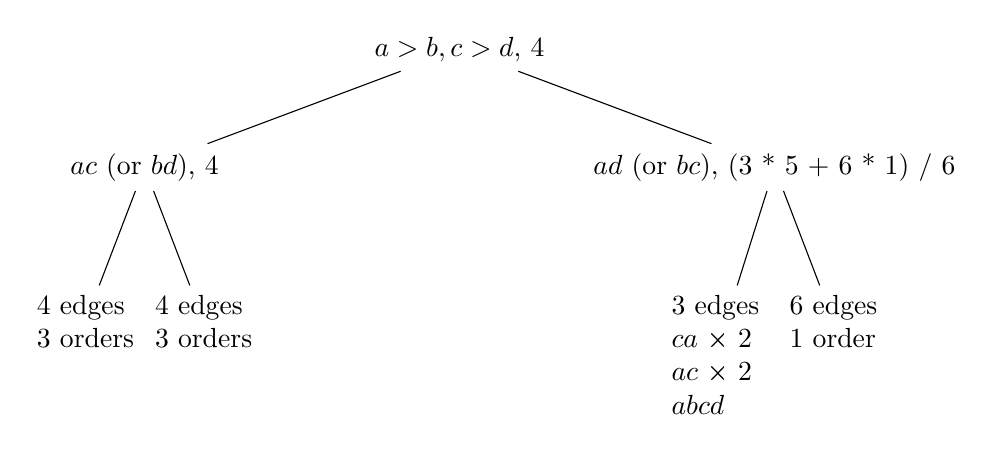
\begin{tikzpicture}
		\path (-10mm, -9mm) coordinate (offsetL);
		\path (10mm, -9mm) coordinate (offsetR);
		\path (0, -4mm) coordinate (offsetG);
		\path [sibling distance = 8cm, level 2/.style = {sibling distance = 1.5cm, align = left, anchor = north}] node[anchor=north] {$a > b, c > d$, \esp{4}}
			child {
				node {$a \relq c$ (or $b \relq d$), \esp{4}}
				child {
					node {
						4 edges\\
						3 orders
					}
				}
				child {
					node {
						4 edges\\
						3 orders
					}
				}
			}
			child {
				node {$a \relq d$ (or $b \relq c$), \esp{(3 * 5 + 6 * 1) / 6}}
				child {
					node {
						3 edges\\
						$ca$ × 2\\
						$ac$ × 2\\
						$abcd$
					}
				}
				child {
					node {
						6 edges\\
						1 order
					}
				}
			}
		;
	\end{tikzpicture}
	\caption{The case $m = 4$, three questions, continued.}
	\label{fig:m4Cont}
\end{figure}

%\bibliography{bibl}

\appendix
\section{Best possible number of edges}
Assume we are the luckiest possible: we can choose the orientation of edges (the answers to questions) so as to maximise the number of resulting edges.

Define the \emph{original graph} as the graph $G$ containing the edge $(a, b)$ iff the question $a \relq b$ was asked and answered with $a > b$. Consider $k < n$. After $k$ questions, $G$ has $k$ edges at best.
The following proposition shows that to maximise the number of edges, it is necessary and sufficient to choose any $k + 1$ vertices and connect them. Note that any graph $G$ with $k$ edges can be uniquely decomposed into components having $k_1$, $k_2$, … edges, with $\sum_i k_i = k$ (in a component, there is a non-oriented path linking any two vertices of the component, and any two components are disconnected).
\begin{proposition}
	Let $G = (\allalts, E)$ be an oriented acyclic graph (not necessarily closed transitively) composed of components having $k_1$, $k_2$, … edges, with $\sum_i k_i = k$.
	Then, its transitive closure $T_G$ has $\binom{k + 1}{2}$ edges iff there is only one component having $k$ edges; otherwise, $T_G$ has less than $\binom{k + 1}{2}$ edges.
\end{proposition}
\begin{proof}[Folklore?]
	In general, $T_G$ has at most $\sum_i \binom{k_i + 1}{2}$ edges. The claim holds because $\binom{k + 1}{2} ≥ \sum_i \binom{k_i + 1}{2}$, with equality iff there is only one component.
	Indeed, the left hand side is half of $(k + 1) k = (\sum_i k_i + 1) \sum_i k_i = (\sum_i k_i)^2 + \sum_i k_i ≥ \sum_i k_i^2 + \sum_i k_i$, with equality iff there is only one component; whereas the right hand side is half of $\sum_i (k_i + 1) k_i = \sum_i k_i^2 + \sum_i k_i$.
\end{proof}

\section{Example context}
$N$ the voters (reviewers), $\card{N} = n$; $X$ the items (articles submitted to a conference), $\card{X} = m$. $PO(X)$ the partially ordered sets over $X$. Let $Q \in PO(X)^N$ represent some partial knowledge of the voters preferences. Consider $f: PO(X)^N → \powersetz{X}$ an enlarged voting rule, that selects winning items on the basis of partial knowledge of the preferences of the voters. Define $f(Q) = \min_{x \in X} \max_{y \in X, (>_{i \in N}) \in compl(Q)} s(y, (>_{i \in N})) - s(x, (>_{i \in N}))$ as selecting the alternatives that minimize the worst regret, where $s$ is the Borda scoring rule (attributing to an alternative at a profile as many points as that alternative beats other alternatives, summed over all voters).

We are interested in asking questions so as to let the regret diminish as fast as possible.
\end{document}

